% docs/minipaper_H2_softsync.tex
\documentclass[11pt]{article}

\usepackage[a4paper,margin=2.6cm]{geometry}
\usepackage{amsmath,amssymb}
\usepackage{graphicx}
\usepackage{booktabs}
\usepackage{hyperref}

\hypersetup{
  colorlinks=true,
  linkcolor=blue,
  citecolor=blue,
  urlcolor=blue
}

\title{E-CFI Demo -- Mini Report (H2): Soft Synchronization and Event-Aware Monitoring}
\author{Internal trace note (repo documentation)}
\date{\today}

\begin{document}
\maketitle

\section{Context}
Step H introduced a minimal, runnable E-CFI simulation with (i) embodied assembly (join/detach), (ii) oscillatory phases, and
(iii) intrinsic signals (novelty/boreness/load). A failure mode observed in some runs is an \emph{absorbing global lock-in}:
once a large assembly forms under hard synchronization, global coherence can saturate near $1$ and remain trivially stable.

\section{H2 goal}
We refine the oscillator/assembly coupling to preserve the \emph{assembly-driven entrainment} semantics while preventing a trivial absorbing regime.
The two H2 interventions are:

\begin{enumerate}
\item \textbf{Soft phase synchronization on merges:} when a join merges two previously disconnected assembly components, phases are not hard-reset;
they are blended toward an anchor phase on the unit circle with a tunable strength $\sigma \in [0,1]$.
\item \textbf{Event-aware monitoring:} the simulation logs per-step join/detach/merge counts, enabling causal reading of changes in
assembly indicators and coherence.
\end{enumerate}

\section{Configuration (run-level contract)}
This report refers to the run:
\begin{itemize}
\item seed: 0
\item $dt = 0.05$, steps $= 3000$
\item $N=50$, torus size $[10,10]$
\item oscillator: $\omega_0 = 0.15$, $\omega_{0,\sigma} = 0.01$, phase noise $=0$
\item \textbf{soft sync strength:} $\sigma = 0.35$ (hard sync corresponds to $\sigma=1$)
\end{itemize}

\section{Implementation note}
Soft synchronization is implemented as a circular (complex) blend:
given current phase $\varphi$ and anchor $\varphi^\star$, with strength $\sigma$,
we map phases to $z = e^{2\pi i \varphi}$, $z^\star = e^{2\pi i \varphi^\star}$ and set
$z_{\text{new}} = (1-\sigma)z + \sigma z^\star$,
then $\varphi_{\text{new}} = \arg(z_{\text{new}})/(2\pi)\ \mathrm{mod}\ 1$.
This avoids discontinuities near $0/1$ and matches the intended circular geometry.

\section{Results: event-aware reading}
Figures \ref{fig:assembly}, \ref{fig:coh}, \ref{fig:events}, and \ref{fig:intrinsic} summarize the run.
Vertical markers indicate merge events (joins that connect two distinct assembly components).

\begin{figure}[t]
\centering
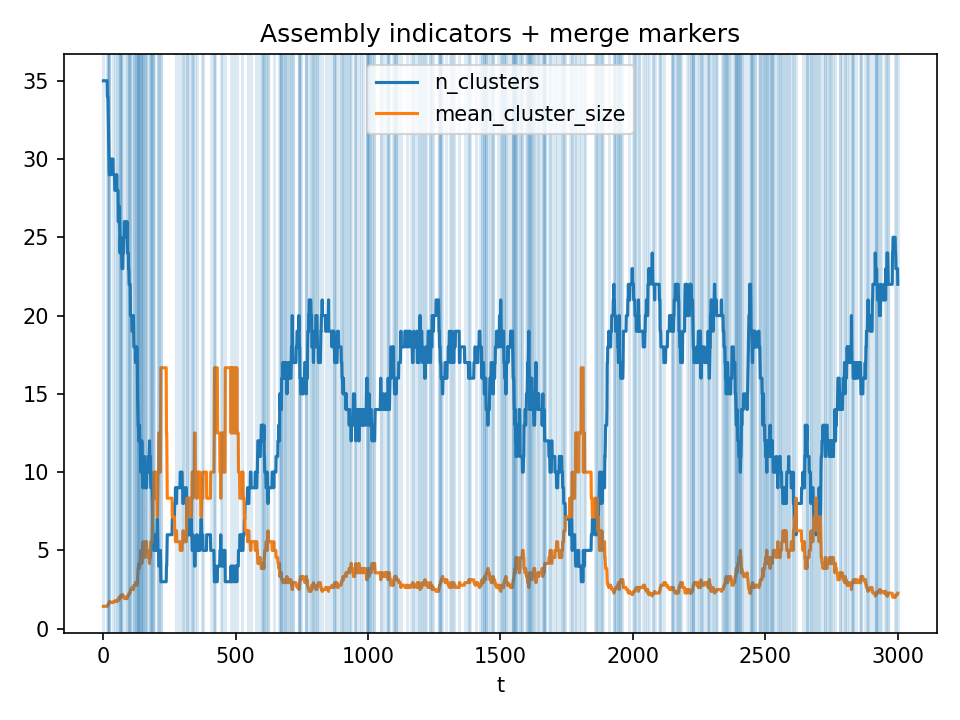
\includegraphics[width=0.92\linewidth]{figures/H2_plot_events_assembly_seed0.png}
\caption{Assembly indicators with merge markers: $n_{\text{clusters}}(t)$ and mean cluster size.}
\label{fig:assembly}
\end{figure}

\begin{figure}[t]
\centering
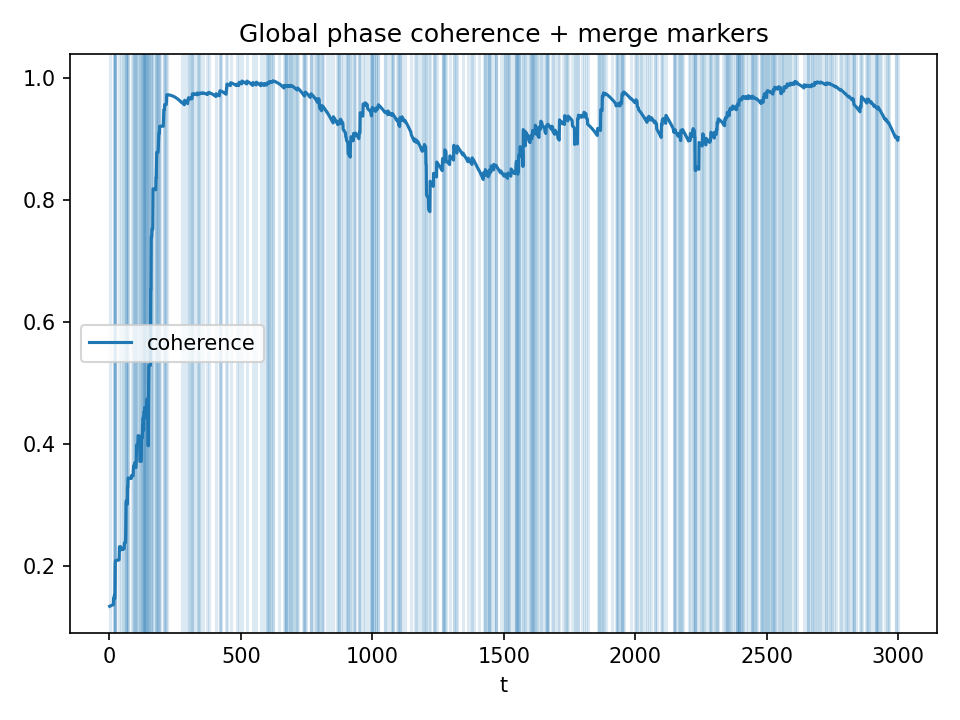
\includegraphics[width=0.92\linewidth]{figures/H2_plot_events_coherence_seed0.png}
\caption{Global phase coherence $r(t)$ with merge markers. Soft sync should prevent permanent saturation at $r=1$ while preserving entrainment at merges.}
\label{fig:coh}
\end{figure}

\begin{figure}[t]
\centering
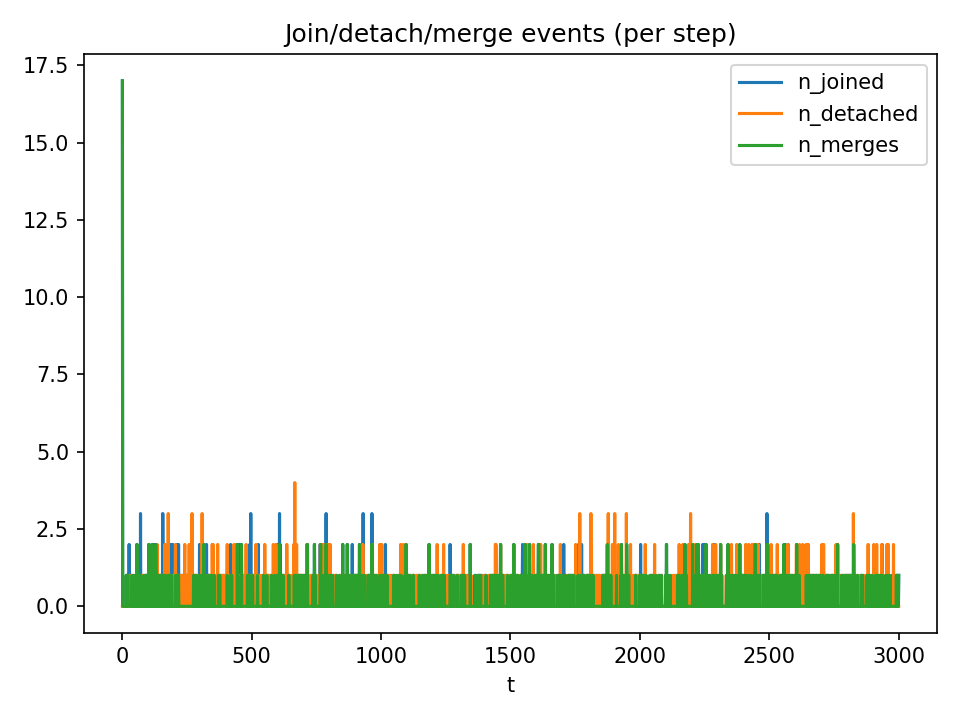
\includegraphics[width=0.92\linewidth]{figures/H2_plot_events_counts_seed0.png}
\caption{Per-step event counts: join, detach, and merge events. These signals support causal interpretation of regime transitions.}
\label{fig:events}
\end{figure}

\begin{figure}[t]
\centering
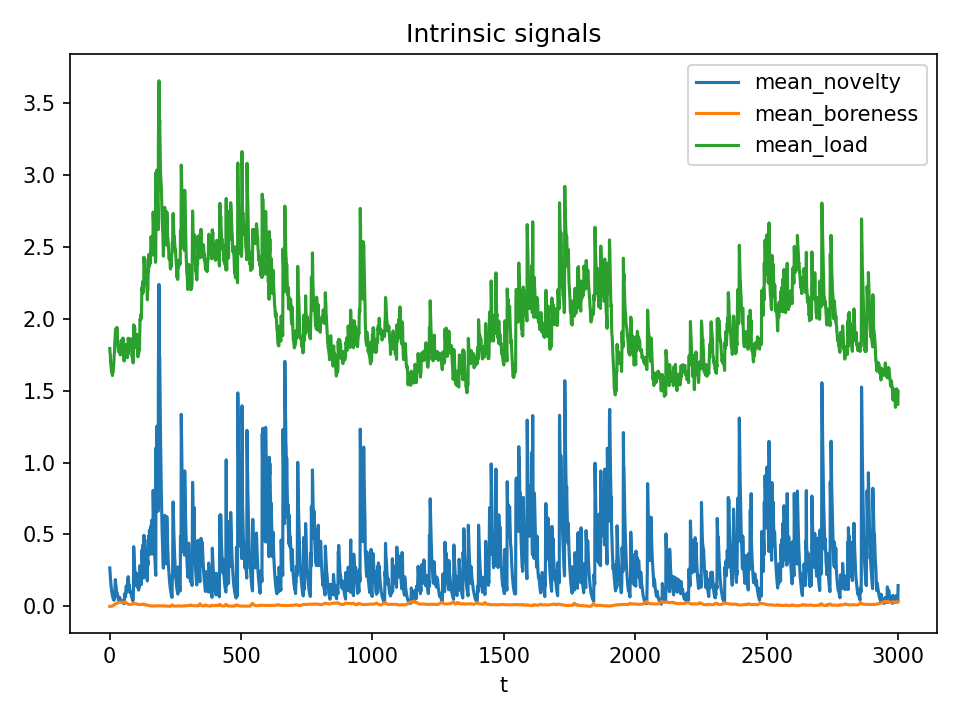
\includegraphics[width=0.92\linewidth]{figures/H2_plot_events_intrinsic_seed0.png}
\caption{Intrinsic signals (means): novelty, boreness, and load.}
\label{fig:intrinsic}
\end{figure}

\section{Interpretive note (what we look for)}
H2 is successful if:
(i) coherence exhibits sustained plateaus and drops that align with detach/merge structure,
(ii) merge events produce coherence increases without enforcing a permanent absorbing lock-in,
(iii) cluster indicators show non-trivial reconfiguration phases supported by intrinsic triggers.

\section{Next step}
If coherence remains overly stable, we will:
(i) decrease $\sigma$ (weaker sync),
(ii) increase $\omega_{0,\sigma}$ slightly (faster drift),
or (iii) introduce \emph{soft sync with rate over multiple steps} rather than an instantaneous blend at merges.

\end{document}